\section{Approach}
\label{sec:approach}

\subsection{Dataset}
Firstly, 
for all the image data from the training dataset~\cite{li2017reliable,li2019reliable}, 
we filter out neutral instances from the original dataset, 
the emotion labels are denoted as 1 (Surprised), 2 (Fearful), 3 (Disgusted), 4 (Happy), 5 (Sad), and 6 (Angry) for simplicity. 
Afterward, 
we transform and resize the images to \texttt{(64,64)}. 

\subsection{Model Architecture}
We implemented an emotion-classification model with 3 convolution layers.

We add a \texttt{dropout} layer to prevent overfitting. 
In order to find the best hyperparameter configuration (see \cref{tab:hyper} for details) of the model, 
we utilize the parameter grid from sklearn~\footnote{\url{https://scikit-learn.org/stable/modules/generated/sklearn.model_selection.ParameterGrid.html}}. 


\begin{table}
    \centering
    \begin{tabular}{@{}lc@{}}
      \toprule
      Hyperparameter & Configuration \\
      \midrule
      Learning rate & \{0.1, 0.01, 0.001, 0.0001\}  \\
      Batch size & \{8, 16, 32, 64\} \\
      Dropout rate & \{0.5\} \\
      Epoch & \{20\} \\
      Early stopping & \{\texttt{True}, \texttt{False}\} \\
      Patience & \{5\} \\
      \bottomrule
    \end{tabular}
    \caption{Explored hyperparameter space for our model}
    \label{tab:hyper}
  \end{table}

\subsection{Preliminary Results}

For evaluation, we use the metric accuracy.

\begin{figure}[ht]
  \centering
  % \fbox{\rule{0pt}{2in} \rule{0.9\linewidth}{0pt}}
   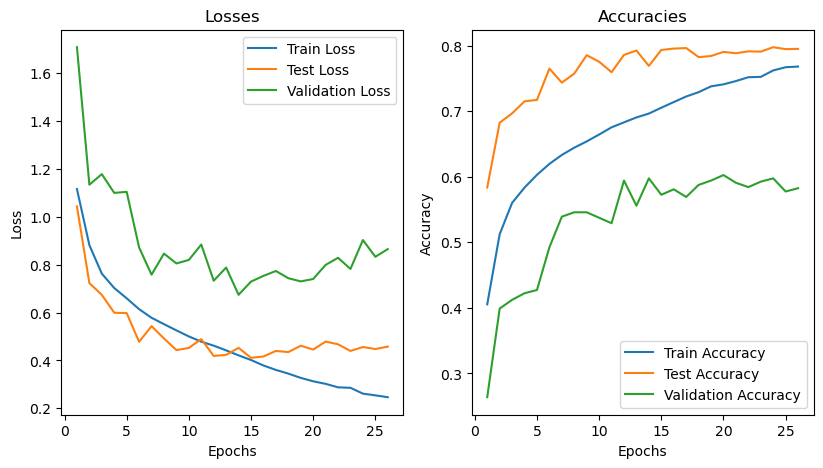
\includegraphics[width=0.95\linewidth]{output.png}
   \caption{Empirical results in terms of the loss and accuracy on differen training epochs}
   \label{fig:result}
\end{figure}

\section*{Acknowledgements}

We are deeply grateful to our advisors \textbf{Johannes Fischer} and \textbf{Ming Gui} for their helpful and valuable support during the entire semester. 
We also thank \textbf{Prof. Dr. Björn Ommer} for providing this interesting practical course.